\documentclass[1p]{elsarticle_modified}
%\bibliographystyle{elsarticle-num}

%\usepackage[colorlinks]{hyperref}
%\usepackage{abbrmath_seonhwa} %\Abb, \Ascr, \Acal ,\Abf, \Afrak
\usepackage{amsfonts}
\usepackage{amssymb}
\usepackage{amsmath}
\usepackage{amsthm}
\usepackage{scalefnt}
\usepackage{amsbsy}
\usepackage{kotex}
\usepackage{caption}
\usepackage{subfig}
\usepackage{color}
\usepackage{graphicx}
\usepackage{xcolor} %% white, black, red, green, blue, cyan, magenta, yellow
\usepackage{float}
\usepackage{setspace}
\usepackage{hyperref}

\usepackage{tikz}
\usetikzlibrary{arrows}

\usepackage{multirow}
\usepackage{array} % fixed length table
\usepackage{hhline}

%%%%%%%%%%%%%%%%%%%%%
\makeatletter
\renewcommand*\env@matrix[1][\arraystretch]{%
	\edef\arraystretch{#1}%
	\hskip -\arraycolsep
	\let\@ifnextchar\new@ifnextchar
	\array{*\c@MaxMatrixCols c}}
\makeatother %https://tex.stackexchange.com/questions/14071/how-can-i-increase-the-line-spacing-in-a-matrix
%%%%%%%%%%%%%%%

\usepackage[normalem]{ulem}

\newcommand{\msout}[1]{\ifmmode\text{\sout{\ensuremath{#1}}}\else\sout{#1}\fi}
%SOURCE: \msout is \stkout macro in https://tex.stackexchange.com/questions/20609/strikeout-in-math-mode

\newcommand{\cancel}[1]{
	\ifmmode
	{\color{red}\msout{#1}}
	\else
	{\color{red}\sout{#1}}
	\fi
}

\newcommand{\add}[1]{
	{\color{blue}\uwave{#1}}
}

\newcommand{\replace}[2]{
	\ifmmode
	{\color{red}\msout{#1}}{\color{blue}\uwave{#2}}
	\else
	{\color{red}\sout{#1}}{\color{blue}\uwave{#2}}
	\fi
}

\newcommand{\Sol}{\mathcal{S}} %segment
\newcommand{\D}{D} %diagram
\newcommand{\A}{\mathcal{A}} %arc


%%%%%%%%%%%%%%%%%%%%%%%%%%%%%5 test

\def\sl{\operatorname{\textup{SL}}(2,\Cbb)}
\def\psl{\operatorname{\textup{PSL}}(2,\Cbb)}
\def\quan{\mkern 1mu \triangleright \mkern 1mu}

\theoremstyle{definition}
\newtheorem{thm}{Theorem}[section]
\newtheorem{prop}[thm]{Proposition}
\newtheorem{lem}[thm]{Lemma}
\newtheorem{ques}[thm]{Question}
\newtheorem{cor}[thm]{Corollary}
\newtheorem{defn}[thm]{Definition}
\newtheorem{exam}[thm]{Example}
\newtheorem{rmk}[thm]{Remark}
\newtheorem{alg}[thm]{Algorithm}

\newcommand{\I}{\sqrt{-1}}
\begin{document}

%\begin{frontmatter}
%
%\title{Boundary parabolic representations of knots up to 8 crossings}
%
%%% Group authors per affiliation:
%\author{Yunhi Cho} 
%\address{Department of Mathematics, University of Seoul, Seoul, Korea}
%\ead{yhcho@uos.ac.kr}
%
%
%\author{Seonhwa Kim} %\fnref{s_kim}}
%\address{Center for Geometry and Physics, Institute for Basic Science, Pohang, 37673, Korea}
%\ead{ryeona17@ibs.re.kr}
%
%\author{Hyuk Kim}
%\address{Department of Mathematical Sciences, Seoul National University, Seoul 08826, Korea}
%\ead{hyukkim@snu.ac.kr}
%
%\author{Seokbeom Yoon}
%\address{Department of Mathematical Sciences, Seoul National University, Seoul, 08826,  Korea}
%\ead{sbyoon15@snu.ac.kr}
%
%\begin{abstract}
%We find all boundary parabolic representation of knots up to 8 crossings.
%
%\end{abstract}
%\begin{keyword}
%    \MSC[2010] 57M25 
%\end{keyword}
%
%\end{frontmatter}

%\linenumbers
%\tableofcontents
%
\newcommand\colored[1]{\textcolor{white}{\rule[-0.35ex]{0.8em}{1.4ex}}\kern-0.8em\color{red} #1}%
%\newcommand\colored[1]{\textcolor{white}{ #1}\kern-2.17ex	\textcolor{white}{ #1}\kern-1.81ex	\textcolor{white}{ #1}\kern-2.15ex\color{red}#1	}

{\Large $\underline{10_{72}~(K10a_{4})}$}

\setlength{\tabcolsep}{10pt}
\renewcommand{\arraystretch}{1.6}
\vspace{1cm}\begin{tabular}{m{100pt}>{\centering\arraybackslash}m{274pt}}
\multirow{5}{120pt}{
	\centering
	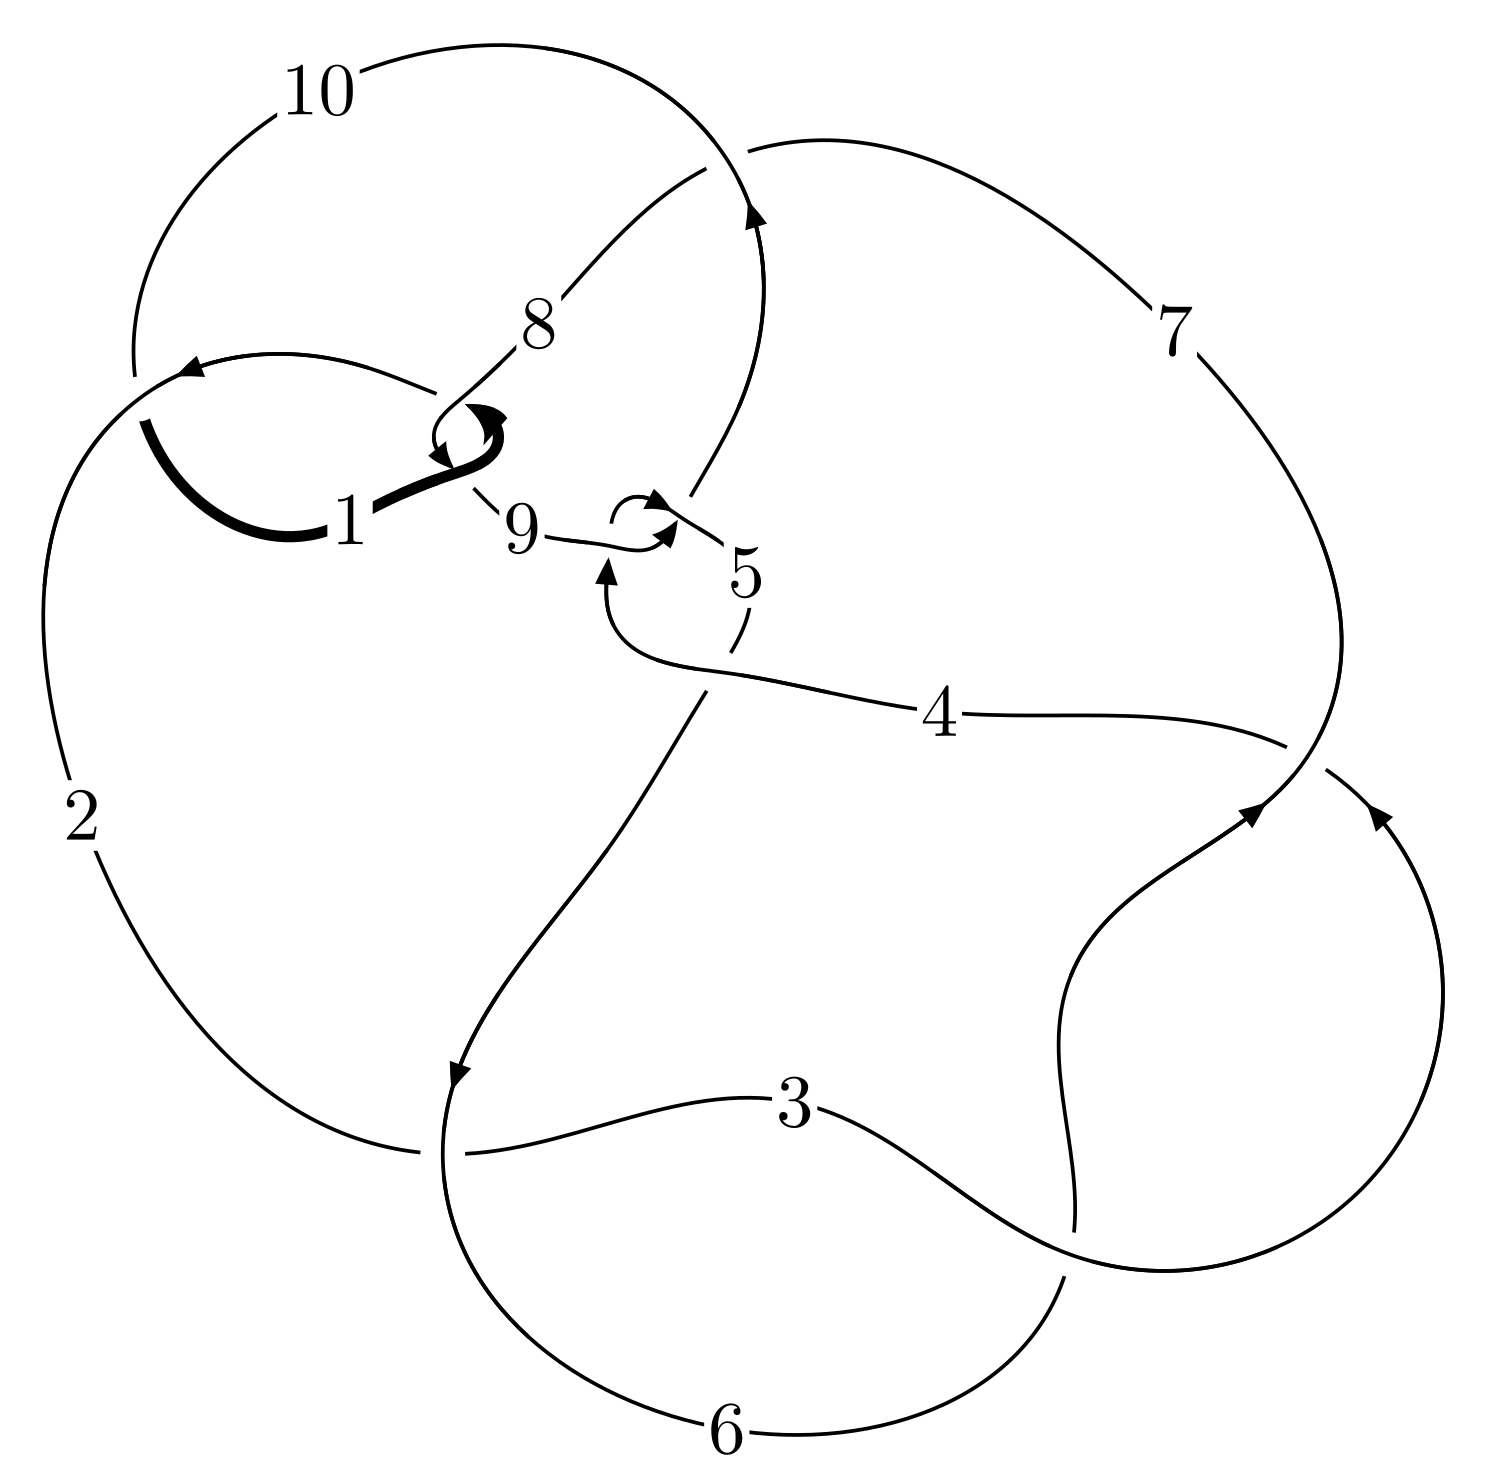
\includegraphics[width=112pt]{../../../GIT/diagram.site/Diagrams/png/156_10_72.png}\\
\ \ \ A knot diagram\footnotemark}&
\allowdisplaybreaks
\textbf{Linearized knot diagam} \\
\cline{2-2}
 &
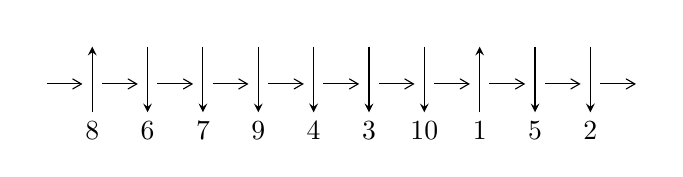
\begin{tikzpicture}[x=20pt, y=17pt]
	% nodes
	\node (C0) at (0, 0) {};
	\node (C1) at (1, 0) {};
	\node (C1U) at (1, +1) {};
	\node (C1D) at (1, -1) {8};

	\node (C2) at (2, 0) {};
	\node (C2U) at (2, +1) {};
	\node (C2D) at (2, -1) {6};

	\node (C3) at (3, 0) {};
	\node (C3U) at (3, +1) {};
	\node (C3D) at (3, -1) {7};

	\node (C4) at (4, 0) {};
	\node (C4U) at (4, +1) {};
	\node (C4D) at (4, -1) {9};

	\node (C5) at (5, 0) {};
	\node (C5U) at (5, +1) {};
	\node (C5D) at (5, -1) {4};

	\node (C6) at (6, 0) {};
	\node (C6U) at (6, +1) {};
	\node (C6D) at (6, -1) {3};

	\node (C7) at (7, 0) {};
	\node (C7U) at (7, +1) {};
	\node (C7D) at (7, -1) {10};

	\node (C8) at (8, 0) {};
	\node (C8U) at (8, +1) {};
	\node (C8D) at (8, -1) {1};

	\node (C9) at (9, 0) {};
	\node (C9U) at (9, +1) {};
	\node (C9D) at (9, -1) {5};

	\node (C10) at (10, 0) {};
	\node (C10U) at (10, +1) {};
	\node (C10D) at (10, -1) {2};
	\node (C11) at (11, 0) {};

	% arrows
	\draw[->,>={angle 60}]
	(C0) edge (C1) (C1) edge (C2) (C2) edge (C3) (C3) edge (C4) (C4) edge (C5) (C5) edge (C6) (C6) edge (C7) (C7) edge (C8) (C8) edge (C9) (C9) edge (C10) (C10) edge (C11) ;	\draw[->,>=stealth]
	(C1D) edge (C1U) (C2U) edge (C2D) (C3U) edge (C3D) (C4U) edge (C4D) (C5U) edge (C5D) (C6U) edge (C6D) (C7U) edge (C7D) (C8D) edge (C8U) (C9U) edge (C9D) (C10U) edge (C10D) ;
	\end{tikzpicture} \\
\hhline{~~} \\& 
\textbf{Solving Sequence} \\ \cline{2-2} 
 &
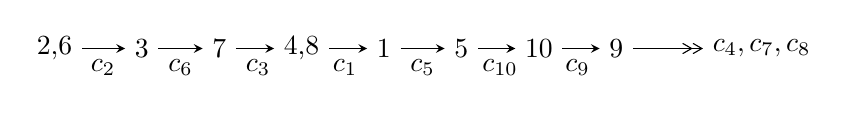
\begin{tikzpicture}[x=28pt, y=7pt]
	% node
	\node (A0) at (-1/8, 0) {2,6};
	\node (A1) at (1, 0) {3};
	\node (A2) at (2, 0) {7};
	\node (A3) at (49/16, 0) {4,8};
	\node (A4) at (33/8, 0) {1};
	\node (A5) at (41/8, 0) {5};
	\node (A6) at (49/8, 0) {10};
	\node (A7) at (57/8, 0) {9};
	\node (C1) at (1/2, -1) {$c_{2}$};
	\node (C2) at (3/2, -1) {$c_{6}$};
	\node (C3) at (5/2, -1) {$c_{3}$};
	\node (C4) at (29/8, -1) {$c_{1}$};
	\node (C5) at (37/8, -1) {$c_{5}$};
	\node (C6) at (45/8, -1) {$c_{10}$};
	\node (C7) at (53/8, -1) {$c_{9}$};
	\node (A8) at (9, 0) {$c_{4},c_{7},c_{8}$};

	% edge
	\draw[->,>=stealth]	
	(A0) edge (A1) (A1) edge (A2) (A2) edge (A3) (A3) edge (A4) (A4) edge (A5) (A5) edge (A6) (A6) edge (A7) ;
	\draw[->>,>={angle 60}]	
	(A7) edge (A8);
\end{tikzpicture} \\ 

\end{tabular} \\

\footnotetext{
The image of knot diagram is generated by the software ``\textbf{Draw programme}" developed by Andrew Bartholomew(\url{http://www.layer8.co.uk/maths/draw/index.htm\#Running-draw}), where we modified some parts for our purpose(\url{https://github.com/CATsTAILs/LinksPainter}).
}\phantom \\ \newline 
\centering \textbf{Ideals for irreducible components\footnotemark of $X_{\text{par}}$} 
 
\begin{align*}
I^u_{1}&=\langle 
u^{37}-2 u^{36}+\cdots+2 b+1,\;- u^{12}+5 u^{10}+2 u^9-9 u^8-8 u^7+4 u^6+10 u^5+6 u^4-2 u^3-5 u^2+a-2 u-1,\\
\phantom{I^u_{1}}&\phantom{= \langle  }u^{38}-3 u^{37}+\cdots+2 u-1\rangle \\
I^u_{2}&=\langle 
b^2- b+1,\;a+1,\;u-1\rangle \\
\\
\end{align*}
\raggedright * 2 irreducible components of $\dim_{\mathbb{C}}=0$, with total 40 representations.\\
\footnotetext{All coefficients of polynomials are rational numbers. But the coefficients are sometimes approximated in decimal forms when there is not enough margin.}
\newpage
\renewcommand{\arraystretch}{1}
\centering \section*{I. $I^u_{1}= \langle u^{37}-2 u^{36}+\cdots+2 b+1,\;- u^{12}+5 u^{10}+\cdots+a-1,\;u^{38}-3 u^{37}+\cdots+2 u-1 \rangle$}
\flushleft \textbf{(i) Arc colorings}\\
\begin{tabular}{m{7pt} m{180pt} m{7pt} m{180pt} }
\flushright $a_{2}=$&$\begin{pmatrix}1\\0\end{pmatrix}$ \\
\flushright $a_{6}=$&$\begin{pmatrix}0\\u\end{pmatrix}$ \\
\flushright $a_{3}=$&$\begin{pmatrix}1\\u^2\end{pmatrix}$ \\
\flushright $a_{7}=$&$\begin{pmatrix}- u\\- u^3+u\end{pmatrix}$ \\
\flushright $a_{4}=$&$\begin{pmatrix}- u^2+1\\- u^4+2 u^2\end{pmatrix}$ \\
\flushright $a_{8}=$&$\begin{pmatrix}u^{12}-5 u^{10}-2 u^9+9 u^8+8 u^7-4 u^6-10 u^5-6 u^4+2 u^3+5 u^2+2 u+1\\-\frac{1}{2} u^{37}+u^{36}+\cdots+\frac{5}{2} u-\frac{1}{2}\end{pmatrix}$ \\
\flushright $a_{1}=$&$\begin{pmatrix}-\frac{1}{2} u^{37}+u^{36}+\cdots+\frac{5}{2} u+\frac{1}{2}\\\frac{5}{2} u^{37}-4 u^{36}+\cdots-\frac{5}{2} u+\frac{3}{2}\end{pmatrix}$ \\
\flushright $a_{5}=$&$\begin{pmatrix}u^5-2 u^3+u\\u^7-3 u^5+2 u^3+u\end{pmatrix}$ \\
\flushright $a_{10}=$&$\begin{pmatrix}2 u^{37}-3 u^{36}+\cdots+10 u^2+2\\\frac{5}{2} u^{37}-4 u^{36}+\cdots-\frac{5}{2} u+\frac{3}{2}\end{pmatrix}$ \\
\flushright $a_{9}=$&$\begin{pmatrix}-3 u^{37}+5 u^{36}+\cdots+5 u-2\\\frac{3}{2} u^{37}-2 u^{36}+\cdots-\frac{1}{2} u+\frac{1}{2}\end{pmatrix}$\\&\end{tabular}
\flushleft \textbf{(ii) Obstruction class $= -1$}\\~\\
\flushleft \textbf{(iii) Cusp Shapes $= -2 u^{37}- u^{36}+35 u^{35}+21 u^{34}-270 u^{33}-205 u^{32}+1194 u^{31}+1182 u^{30}-3222 u^{29}-4364 u^{28}+4873 u^{27}+10507 u^{26}-1460 u^{25}-15693 u^{24}-9964 u^{23}+11016 u^{22}+21182 u^{21}+5747 u^{20}-16959 u^{19}-19349 u^{18}-2018 u^{17}+13493 u^{16}+13726 u^{15}+2674 u^{14}-6790 u^{13}-7586 u^{12}-3020 u^{11}+1300 u^{10}+2786 u^9+1852 u^8+442 u^7-314 u^6-448 u^5-263 u^4-91 u^3-25 u^2+4 u-5$}\\~\\
\newpage\renewcommand{\arraystretch}{1}
\flushleft \textbf{(iv) u-Polynomials at the component}\newline \\
\begin{tabular}{m{50pt}|m{274pt}}
Crossings & \hspace{64pt}u-Polynomials at each crossing \\
\hline $$\begin{aligned}c_{1},c_{8}\end{aligned}$$&$\begin{aligned}
&u^{38}+2 u^{37}+\cdots+5 u+1
\end{aligned}$\\
\hline $$\begin{aligned}c_{2},c_{3},c_{6}\end{aligned}$$&$\begin{aligned}
&u^{38}-3 u^{37}+\cdots+2 u-1
\end{aligned}$\\
\hline $$\begin{aligned}c_{4},c_{9}\end{aligned}$$&$\begin{aligned}
&u^{38}- u^{37}+\cdots-4 u-4
\end{aligned}$\\
\hline $$\begin{aligned}c_{5}\end{aligned}$$&$\begin{aligned}
&u^{38}+15 u^{37}+\cdots+72 u+16
\end{aligned}$\\
\hline $$\begin{aligned}c_{7}\end{aligned}$$&$\begin{aligned}
&u^{38}-2 u^{37}+\cdots-37 u+17
\end{aligned}$\\
\hline $$\begin{aligned}c_{10}\end{aligned}$$&$\begin{aligned}
&u^{38}+18 u^{37}+\cdots-5 u+1
\end{aligned}$\\
\hline
\end{tabular}\\~\\
\newpage\renewcommand{\arraystretch}{1}
\flushleft \textbf{(v) Riley Polynomials at the component}\newline \\
\begin{tabular}{m{50pt}|m{274pt}}
Crossings & \hspace{64pt}Riley Polynomials at each crossing \\
\hline $$\begin{aligned}c_{1},c_{8}\end{aligned}$$&$\begin{aligned}
&y^{38}+18 y^{37}+\cdots-5 y+1
\end{aligned}$\\
\hline $$\begin{aligned}c_{2},c_{3},c_{6}\end{aligned}$$&$\begin{aligned}
&y^{38}-33 y^{37}+\cdots-8 y+1
\end{aligned}$\\
\hline $$\begin{aligned}c_{4},c_{9}\end{aligned}$$&$\begin{aligned}
&y^{38}-15 y^{37}+\cdots-72 y+16
\end{aligned}$\\
\hline $$\begin{aligned}c_{5}\end{aligned}$$&$\begin{aligned}
&y^{38}+13 y^{37}+\cdots-2848 y+256
\end{aligned}$\\
\hline $$\begin{aligned}c_{7}\end{aligned}$$&$\begin{aligned}
&y^{38}-6 y^{37}+\cdots-6333 y+289
\end{aligned}$\\
\hline $$\begin{aligned}c_{10}\end{aligned}$$&$\begin{aligned}
&y^{38}+6 y^{37}+\cdots-61 y+1
\end{aligned}$\\
\hline
\end{tabular}\\~\\
\newpage\flushleft \textbf{(vi) Complex Volumes and Cusp Shapes}
$$\begin{array}{c|c|c}  
\text{Solutions to }I^u_{1}& \I (\text{vol} + \sqrt{-1}CS) & \text{Cusp shape}\\
 \hline 
\begin{aligned}
u &= -1.000620 + 0.466336 I \\
a &= \phantom{-}0.694761 - 0.337574 I \\
b &= -0.527298 + 1.065360 I\end{aligned}
 & -2.40471 - 3.95746 I & -10.27520 + 4.57056 I \\ \hline\begin{aligned}
u &= -1.000620 - 0.466336 I \\
a &= \phantom{-}0.694761 + 0.337574 I \\
b &= -0.527298 - 1.065360 I\end{aligned}
 & -2.40471 + 3.95746 I & -10.27520 - 4.57056 I \\ \hline\begin{aligned}
u &= -1.062270 + 0.332916 I \\
a &= \phantom{-}1.252160 - 0.030949 I \\
b &= -0.570085 - 0.447308 I\end{aligned}
 & -0.568983 + 0.479860 I & -6.06539 + 0.48126 I \\ \hline\begin{aligned}
u &= -1.062270 - 0.332916 I \\
a &= \phantom{-}1.252160 + 0.030949 I \\
b &= -0.570085 + 0.447308 I\end{aligned}
 & -0.568983 - 0.479860 I & -6.06539 - 0.48126 I \\ \hline\begin{aligned}
u &= -0.719303 + 0.499357 I \\
a &= \phantom{-}1.44677 - 0.15075 I \\
b &= -0.362704 - 1.048010 I\end{aligned}
 & -3.54227 + 2.75914 I & -13.19764 - 4.35912 I \\ \hline\begin{aligned}
u &= -0.719303 - 0.499357 I \\
a &= \phantom{-}1.44677 + 0.15075 I \\
b &= -0.362704 + 1.048010 I\end{aligned}
 & -3.54227 - 2.75914 I & -13.19764 + 4.35912 I \\ \hline\begin{aligned}
u &= -0.214521 + 0.842165 I \\
a &= \phantom{-}2.14112 + 0.49356 I \\
b &= -0.573770 - 1.100590 I\end{aligned}
 & \phantom{-}0.00579 + 8.62980 I & -6.60829 - 7.80256 I \\ \hline\begin{aligned}
u &= -0.214521 - 0.842165 I \\
a &= \phantom{-}2.14112 - 0.49356 I \\
b &= -0.573770 + 1.100590 I\end{aligned}
 & \phantom{-}0.00579 - 8.62980 I & -6.60829 + 7.80256 I \\ \hline\begin{aligned}
u &= -0.174468 + 0.788088 I \\
a &= \phantom{-}1.39685 - 0.95450 I \\
b &= -0.731729 + 0.388434 I\end{aligned}
 & \phantom{-}2.09675 + 3.65224 I & -3.04639 - 3.74887 I \\ \hline\begin{aligned}
u &= -0.174468 - 0.788088 I \\
a &= \phantom{-}1.39685 + 0.95450 I \\
b &= -0.731729 - 0.388434 I\end{aligned}
 & \phantom{-}2.09675 - 3.65224 I & -3.04639 + 3.74887 I\\
 \hline 
 \end{array}$$\newpage$$\begin{array}{c|c|c}  
\text{Solutions to }I^u_{1}& \I (\text{vol} + \sqrt{-1}CS) & \text{Cusp shape}\\
 \hline 
\begin{aligned}
u &= -0.317784 + 0.691757 I \\
a &= \phantom{-}0.058360 - 0.565761 I \\
b &= -0.214760 + 1.058960 I\end{aligned}
 & -2.35641 + 1.43399 I & -10.35352 - 2.88902 I \\ \hline\begin{aligned}
u &= -0.317784 - 0.691757 I \\
a &= \phantom{-}0.058360 + 0.565761 I \\
b &= -0.214760 - 1.058960 I\end{aligned}
 & -2.35641 - 1.43399 I & -10.35352 + 2.88902 I \\ \hline\begin{aligned}
u &= \phantom{-}1.251800 + 0.201783 I \\
a &= -0.999363 - 0.281232 I \\
b &= \phantom{-}0.652278 + 0.954226 I\end{aligned}
 & -2.15443 + 0.39089 I & -9.84825 + 1.14697 I \\ \hline\begin{aligned}
u &= \phantom{-}1.251800 - 0.201783 I \\
a &= -0.999363 + 0.281232 I \\
b &= \phantom{-}0.652278 - 0.954226 I\end{aligned}
 & -2.15443 - 0.39089 I & -9.84825 - 1.14697 I \\ \hline\begin{aligned}
u &= -1.260340 + 0.253559 I \\
a &= -0.003037 + 0.946509 I \\
b &= \phantom{-}0.662945 - 0.361405 I\end{aligned}
 & -1.02515 + 1.90334 I & -5.81979 - 1.07076 I \\ \hline\begin{aligned}
u &= -1.260340 - 0.253559 I \\
a &= -0.003037 - 0.946509 I \\
b &= \phantom{-}0.662945 + 0.361405 I\end{aligned}
 & -1.02515 - 1.90334 I & -5.81979 + 1.07076 I \\ \hline\begin{aligned}
u &= \phantom{-}1.284790 + 0.261207 I \\
a &= -1.278000 + 0.104536 I \\
b &= \phantom{-}0.731652 - 0.644131 I\end{aligned}
 & -1.23963 - 4.86305 I & -7.46881 + 6.13263 I \\ \hline\begin{aligned}
u &= \phantom{-}1.284790 - 0.261207 I \\
a &= -1.278000 - 0.104536 I \\
b &= \phantom{-}0.731652 + 0.644131 I\end{aligned}
 & -1.23963 + 4.86305 I & -7.46881 - 6.13263 I \\ \hline\begin{aligned}
u &= -0.016707 + 0.678781 I \\
a &= -1.38023 - 1.35662 I \\
b &= \phantom{-}0.666801 + 0.530991 I\end{aligned}
 & \phantom{-}2.80379 + 1.46931 I & -1.12935 - 3.08473 I \\ \hline\begin{aligned}
u &= -0.016707 - 0.678781 I \\
a &= -1.38023 + 1.35662 I \\
b &= \phantom{-}0.666801 - 0.530991 I\end{aligned}
 & \phantom{-}2.80379 - 1.46931 I & -1.12935 + 3.08473 I\\
 \hline 
 \end{array}$$\newpage$$\begin{array}{c|c|c}  
\text{Solutions to }I^u_{1}& \I (\text{vol} + \sqrt{-1}CS) & \text{Cusp shape}\\
 \hline 
\begin{aligned}
u &= -1.315510 + 0.121395 I \\
a &= \phantom{-}0.61655 - 1.44009 I \\
b &= \phantom{-}0.291142 - 1.061280 I\end{aligned}
 & -4.89567 - 0.49664 I & -12.27278 + 1.11503 I \\ \hline\begin{aligned}
u &= -1.315510 - 0.121395 I \\
a &= \phantom{-}0.61655 + 1.44009 I \\
b &= \phantom{-}0.291142 + 1.061280 I\end{aligned}
 & -4.89567 + 0.49664 I & -12.27278 - 1.11503 I \\ \hline\begin{aligned}
u &= -1.329280 + 0.259672 I \\
a &= -1.99856 + 1.39234 I \\
b &= \phantom{-}0.547737 + 1.093970 I\end{aligned}
 & -3.13917 + 6.61979 I & -9.45062 - 5.39938 I \\ \hline\begin{aligned}
u &= -1.329280 - 0.259672 I \\
a &= -1.99856 - 1.39234 I \\
b &= \phantom{-}0.547737 - 1.093970 I\end{aligned}
 & -3.13917 - 6.61979 I & -9.45062 + 5.39938 I \\ \hline\begin{aligned}
u &= \phantom{-}0.091958 + 0.636482 I \\
a &= -2.64958 + 0.37806 I \\
b &= \phantom{-}0.571517 - 1.023410 I\end{aligned}
 & \phantom{-}1.34864 - 3.34557 I & -3.46602 + 2.94107 I \\ \hline\begin{aligned}
u &= \phantom{-}0.091958 - 0.636482 I \\
a &= -2.64958 - 0.37806 I \\
b &= \phantom{-}0.571517 + 1.023410 I\end{aligned}
 & \phantom{-}1.34864 + 3.34557 I & -3.46602 - 2.94107 I \\ \hline\begin{aligned}
u &= \phantom{-}1.372870 + 0.330158 I \\
a &= \phantom{-}0.451776 + 0.876637 I \\
b &= -0.811572 - 0.358412 I\end{aligned}
 & -2.79986 - 7.69321 I & \phantom{-0.000000 } 0 \\ \hline\begin{aligned}
u &= \phantom{-}1.372870 - 0.330158 I \\
a &= \phantom{-}0.451776 - 0.876637 I \\
b &= -0.811572 + 0.358412 I\end{aligned}
 & -2.79986 + 7.69321 I & \phantom{-0.000000 } 0 \\ \hline\begin{aligned}
u &= -0.582954\phantom{ +0.000000I} \\
a &= \phantom{-}0.891810\phantom{ +0.000000I} \\
b &= -0.340706\phantom{ +0.000000I}\end{aligned}
 & -0.970134\phantom{ +0.000000I} & -9.92360\phantom{ +0.000000I} \\ \hline\begin{aligned}
u &= \phantom{-}1.42045\phantom{ +0.000000I} \\
a &= \phantom{-}0.242047\phantom{ +0.000000I} \\
b &= -0.758415\phantom{ +0.000000I}\end{aligned}
 & -7.33419\phantom{ +0.000000I} & -11.4900\phantom{ +0.000000I}\\
 \hline 
 \end{array}$$\newpage$$\begin{array}{c|c|c}  
\text{Solutions to }I^u_{1}& \I (\text{vol} + \sqrt{-1}CS) & \text{Cusp shape}\\
 \hline 
\begin{aligned}
u &= \phantom{-}1.40646 + 0.27352 I \\
a &= -0.517124 - 0.625628 I \\
b &= -0.183991 - 1.166970 I\end{aligned}
 & -7.80695 - 4.93169 I & \phantom{-0.000000 } 0 \\ \hline\begin{aligned}
u &= \phantom{-}1.40646 - 0.27352 I \\
a &= -0.517124 + 0.625628 I \\
b &= -0.183991 + 1.166970 I\end{aligned}
 & -7.80695 + 4.93169 I & \phantom{-0.000000 } 0 \\ \hline\begin{aligned}
u &= \phantom{-}1.39814 + 0.35135 I \\
a &= \phantom{-}1.96262 + 0.82883 I \\
b &= -0.591496 + 1.133850 I\end{aligned}
 & -5.10692 - 12.92960 I & \phantom{-0.000000 } 0 \\ \hline\begin{aligned}
u &= \phantom{-}1.39814 - 0.35135 I \\
a &= \phantom{-}1.96262 - 0.82883 I \\
b &= -0.591496 - 1.133850 I\end{aligned}
 & -5.10692 + 12.92960 I & \phantom{-0.000000 } 0 \\ \hline\begin{aligned}
u &= \phantom{-}1.47061 + 0.05198 I \\
a &= \phantom{-}0.671770 + 1.172880 I \\
b &= -0.422515 + 1.169490 I\end{aligned}
 & -10.78740 - 4.17106 I & \phantom{-0.000000 } 0 \\ \hline\begin{aligned}
u &= \phantom{-}1.47061 - 0.05198 I \\
a &= \phantom{-}0.671770 - 1.172880 I \\
b &= -0.422515 - 1.169490 I\end{aligned}
 & -10.78740 + 4.17106 I & \phantom{-0.000000 } 0 \\ \hline\begin{aligned}
u &= \phantom{-}0.215436 + 0.157466 I \\
a &= \phantom{-}1.56623 + 0.67273 I \\
b &= \phantom{-}0.415410 + 0.878457 I\end{aligned}
 & -0.33342 + 1.74546 I & -2.32569 - 3.49934 I \\ \hline\begin{aligned}
u &= \phantom{-}0.215436 - 0.157466 I \\
a &= \phantom{-}1.56623 - 0.67273 I \\
b &= \phantom{-}0.415410 - 0.878457 I\end{aligned}
 & -0.33342 - 1.74546 I & -2.32569 + 3.49934 I\\
 \hline 
 \end{array}$$\newpage\newpage\renewcommand{\arraystretch}{1}
\centering \section*{II. $I^u_{2}= \langle b^2- b+1,\;a+1,\;u-1 \rangle$}
\flushleft \textbf{(i) Arc colorings}\\
\begin{tabular}{m{7pt} m{180pt} m{7pt} m{180pt} }
\flushright $a_{2}=$&$\begin{pmatrix}1\\0\end{pmatrix}$ \\
\flushright $a_{6}=$&$\begin{pmatrix}0\\1\end{pmatrix}$ \\
\flushright $a_{3}=$&$\begin{pmatrix}1\\1\end{pmatrix}$ \\
\flushright $a_{7}=$&$\begin{pmatrix}-1\\0\end{pmatrix}$ \\
\flushright $a_{4}=$&$\begin{pmatrix}0\\1\end{pmatrix}$ \\
\flushright $a_{8}=$&$\begin{pmatrix}-1\\b\end{pmatrix}$ \\
\flushright $a_{1}=$&$\begin{pmatrix}- b+1\\b-1\end{pmatrix}$ \\
\flushright $a_{5}=$&$\begin{pmatrix}0\\1\end{pmatrix}$ \\
\flushright $a_{10}=$&$\begin{pmatrix}0\\b-1\end{pmatrix}$ \\
\flushright $a_{9}=$&$\begin{pmatrix}0\\b-1\end{pmatrix}$\\&\end{tabular}
\flushleft \textbf{(ii) Obstruction class $= 1$}\\~\\
\flushleft \textbf{(iii) Cusp Shapes $= -4 b-7$}\\~\\
\newpage\renewcommand{\arraystretch}{1}
\flushleft \textbf{(iv) u-Polynomials at the component}\newline \\
\begin{tabular}{m{50pt}|m{274pt}}
Crossings & \hspace{64pt}u-Polynomials at each crossing \\
\hline $$\begin{aligned}c_{1},c_{7},c_{10}\end{aligned}$$&$\begin{aligned}
&u^2- u+1
\end{aligned}$\\
\hline $$\begin{aligned}c_{2},c_{3}\end{aligned}$$&$\begin{aligned}
&(u-1)^2
\end{aligned}$\\
\hline $$\begin{aligned}c_{4},c_{5},c_{9}\end{aligned}$$&$\begin{aligned}
&u^2
\end{aligned}$\\
\hline $$\begin{aligned}c_{6}\end{aligned}$$&$\begin{aligned}
&(u+1)^2
\end{aligned}$\\
\hline $$\begin{aligned}c_{8}\end{aligned}$$&$\begin{aligned}
&u^2+u+1
\end{aligned}$\\
\hline
\end{tabular}\\~\\
\newpage\renewcommand{\arraystretch}{1}
\flushleft \textbf{(v) Riley Polynomials at the component}\newline \\
\begin{tabular}{m{50pt}|m{274pt}}
Crossings & \hspace{64pt}Riley Polynomials at each crossing \\
\hline $$\begin{aligned}c_{1},c_{7},c_{8}\\c_{10}\end{aligned}$$&$\begin{aligned}
&y^2+y+1
\end{aligned}$\\
\hline $$\begin{aligned}c_{2},c_{3},c_{6}\end{aligned}$$&$\begin{aligned}
&(y-1)^2
\end{aligned}$\\
\hline $$\begin{aligned}c_{4},c_{5},c_{9}\end{aligned}$$&$\begin{aligned}
&y^2
\end{aligned}$\\
\hline
\end{tabular}\\~\\
\newpage\flushleft \textbf{(vi) Complex Volumes and Cusp Shapes}
$$\begin{array}{c|c|c}  
\text{Solutions to }I^u_{2}& \I (\text{vol} + \sqrt{-1}CS) & \text{Cusp shape}\\
 \hline 
\begin{aligned}
u &= \phantom{-}1.00000\phantom{ +0.000000I} \\
a &= -1.00000\phantom{ +0.000000I} \\
b &= \phantom{-}0.500000 + 0.866025 I\end{aligned}
 & -1.64493 + 2.02988 I & -9.00000 - 3.46410 I \\ \hline\begin{aligned}
u &= \phantom{-}1.00000\phantom{ +0.000000I} \\
a &= -1.00000\phantom{ +0.000000I} \\
b &= \phantom{-}0.500000 - 0.866025 I\end{aligned}
 & -1.64493 - 2.02988 I & -9.00000 + 3.46410 I\\
 \hline 
 \end{array}$$\newpage
\newpage\renewcommand{\arraystretch}{1}
\centering \section*{ III. u-Polynomials}
\begin{tabular}{m{50pt}|m{274pt}}
Crossings & \hspace{64pt}u-Polynomials at each crossing \\
\hline $$\begin{aligned}c_{1}\end{aligned}$$&$\begin{aligned}
&(u^2- u+1)(u^{38}+2 u^{37}+\cdots+5 u+1)
\end{aligned}$\\
\hline $$\begin{aligned}c_{2},c_{3}\end{aligned}$$&$\begin{aligned}
&((u-1)^2)(u^{38}-3 u^{37}+\cdots+2 u-1)
\end{aligned}$\\
\hline $$\begin{aligned}c_{4},c_{9}\end{aligned}$$&$\begin{aligned}
&u^2(u^{38}- u^{37}+\cdots-4 u-4)
\end{aligned}$\\
\hline $$\begin{aligned}c_{5}\end{aligned}$$&$\begin{aligned}
&u^2(u^{38}+15 u^{37}+\cdots+72 u+16)
\end{aligned}$\\
\hline $$\begin{aligned}c_{6}\end{aligned}$$&$\begin{aligned}
&((u+1)^2)(u^{38}-3 u^{37}+\cdots+2 u-1)
\end{aligned}$\\
\hline $$\begin{aligned}c_{7}\end{aligned}$$&$\begin{aligned}
&(u^2- u+1)(u^{38}-2 u^{37}+\cdots-37 u+17)
\end{aligned}$\\
\hline $$\begin{aligned}c_{8}\end{aligned}$$&$\begin{aligned}
&(u^2+u+1)(u^{38}+2 u^{37}+\cdots+5 u+1)
\end{aligned}$\\
\hline $$\begin{aligned}c_{10}\end{aligned}$$&$\begin{aligned}
&(u^2- u+1)(u^{38}+18 u^{37}+\cdots-5 u+1)
\end{aligned}$\\
\hline
\end{tabular}\newpage\renewcommand{\arraystretch}{1}
\centering \section*{ IV. Riley Polynomials}
\begin{tabular}{m{50pt}|m{274pt}}
Crossings & \hspace{64pt}Riley Polynomials at each crossing \\
\hline $$\begin{aligned}c_{1},c_{8}\end{aligned}$$&$\begin{aligned}
&(y^2+y+1)(y^{38}+18 y^{37}+\cdots-5 y+1)
\end{aligned}$\\
\hline $$\begin{aligned}c_{2},c_{3},c_{6}\end{aligned}$$&$\begin{aligned}
&((y-1)^2)(y^{38}-33 y^{37}+\cdots-8 y+1)
\end{aligned}$\\
\hline $$\begin{aligned}c_{4},c_{9}\end{aligned}$$&$\begin{aligned}
&y^2(y^{38}-15 y^{37}+\cdots-72 y+16)
\end{aligned}$\\
\hline $$\begin{aligned}c_{5}\end{aligned}$$&$\begin{aligned}
&y^2(y^{38}+13 y^{37}+\cdots-2848 y+256)
\end{aligned}$\\
\hline $$\begin{aligned}c_{7}\end{aligned}$$&$\begin{aligned}
&(y^2+y+1)(y^{38}-6 y^{37}+\cdots-6333 y+289)
\end{aligned}$\\
\hline $$\begin{aligned}c_{10}\end{aligned}$$&$\begin{aligned}
&(y^2+y+1)(y^{38}+6 y^{37}+\cdots-61 y+1)
\end{aligned}$\\
\hline
\end{tabular}
\vskip 2pc
\end{document}